We decided to develop a mobile application to create a system that can implement the fingerprinting technique in a suitable way.
The benefit of using a mobile application is that typical mobile devices already have the capability to interact and collect data from Bluetooth devices, such as Bluetooth beacons. 
This allowed us to integrate the process of collecting the data, doing classification, and applying the resulting classification model to conduct experiments within the same system.

The application will be developed in C#\cite{billwagnerDocsGetStarted} with Blazor\cite{BlazorBuildClient} and Razor Pages\cite{tdykstraIntroductionRazorPages2023}.

A primary function of the application is to collect data from the aforementioned beacons. 
As illustrated in figure \ref{fig:ScanAdvertisement}, when the device is running, it will scan for advertisement packets broadcast by the Bluetooth beacons.

\begin{figure}[H]
    \centering
    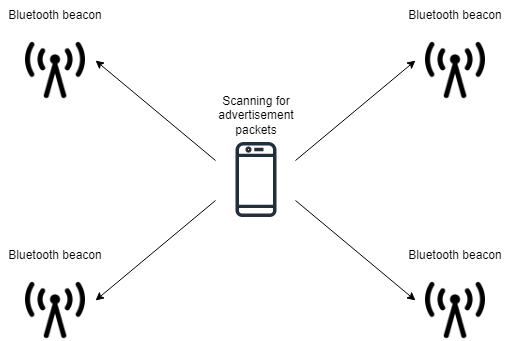
\includegraphics[width=0.5\textwidth]{images/ScanningForAdvertisement.drawio.png}
    \caption{Illustrating a mobile device scanning for Bluetooth beacons}
    \label{fig:ScanAdvertisement}
\end{figure}

Each beacon broadcasts data, which may include a unique identifier for the specific beacon or manufacturer-specific information.
A device configured to receive these broadcasts can extract this information and also calculate the received signal strength indicator (RSSI) of the signal.

As outlined in section \ref{sec:fingerprinting}, fingerprinting involves two stages.
The first stage entails the creation of a map based on the RSSI of the received Bluetooth signal. The second stage involves estimating the unknown location of a Bluetooth receiver.

Through the collection of the broadcast data from the beacons, the application supports the initial phase of fingerprinting, which involves map generation.
Figure \ref{fig:CreateMap} illustrates the map creation process. During this process, a device equipped with the application collects data while being carried around the room in a specific pattern.

Moreover, the beacons are strategically positioned to demarcate the room's perimeter, a critical aspect in the second stage, which entails position inference.

\begin{figure}[H]
    \centering
    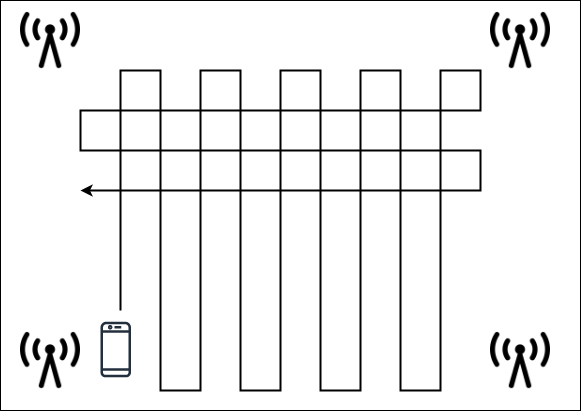
\includegraphics[width=0.5\textwidth]{images/CreateMap.drawio.png}
    \caption{Illustrating a mobile device collecting data from Bluetooth beacons}
    \label{fig:CreateMap}
\end{figure}

To support the second phase of fingerprinting, we have developed a classification module as part of the application. 
By collecting new data and using the map generated during the first phase, the classification module is able to classify the position of other devices relative to the room. 
Using the classifier, the application is able to estimate whether a device is either inside or outside the room.

The system diagram in figure \ref{fig:implementation_diagram} illustrates the system architecture and design.
In the following sections, we delve deeper into each phase, offering comprehensive descriptions of crucial aspects of the implementation. In addition, we present our reasoning behind our chosen methodology.

\begin{figure}[H]
  \centering
  \rotatebox{90}{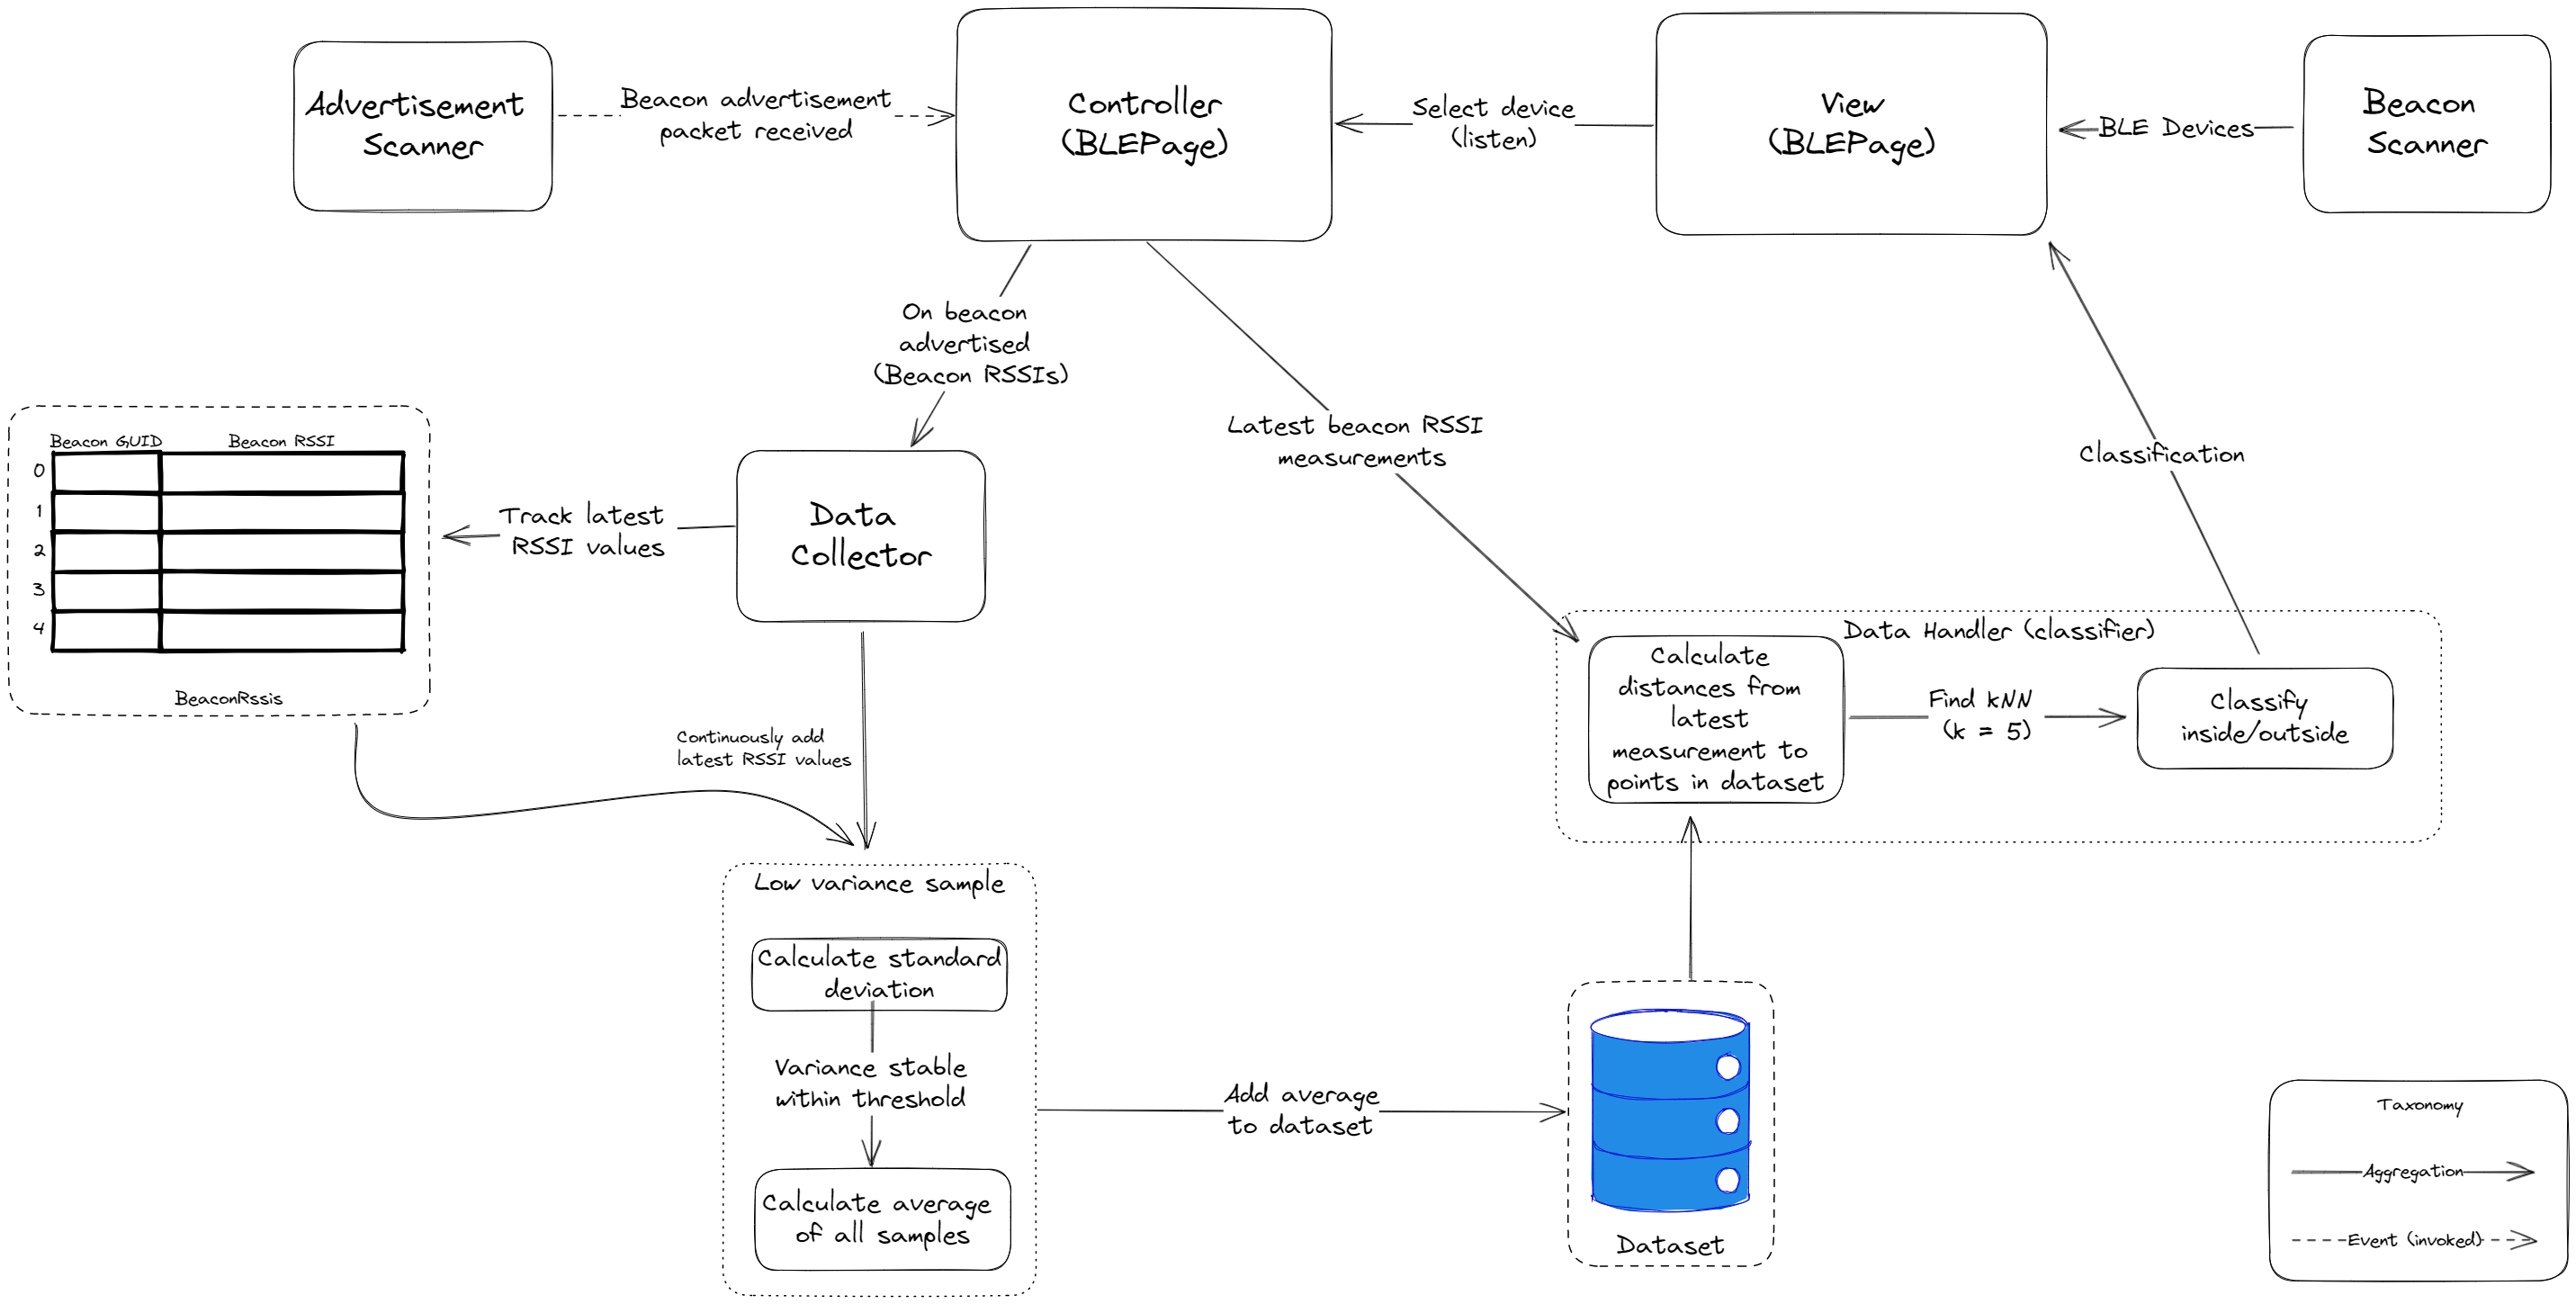
\includegraphics[width=1.75\textwidth]{images/implementation-diagram.png}}
  \caption{Diagram showing the implementation of the system}
  \label{fig:implementation_diagram}
\end{figure}